\section{Исследовательский раздел}

\subsection{Результаты работы разработанного ПО}

На рисунках \ref{fig:example_mem}-\ref{fig:example_syscalls} представлены примеры работы модуля (статистика по количеству свободной и занятой оперативной памяти и по количеству системных вызовов).

\begin{figure}[h!]
	\begin{center}
		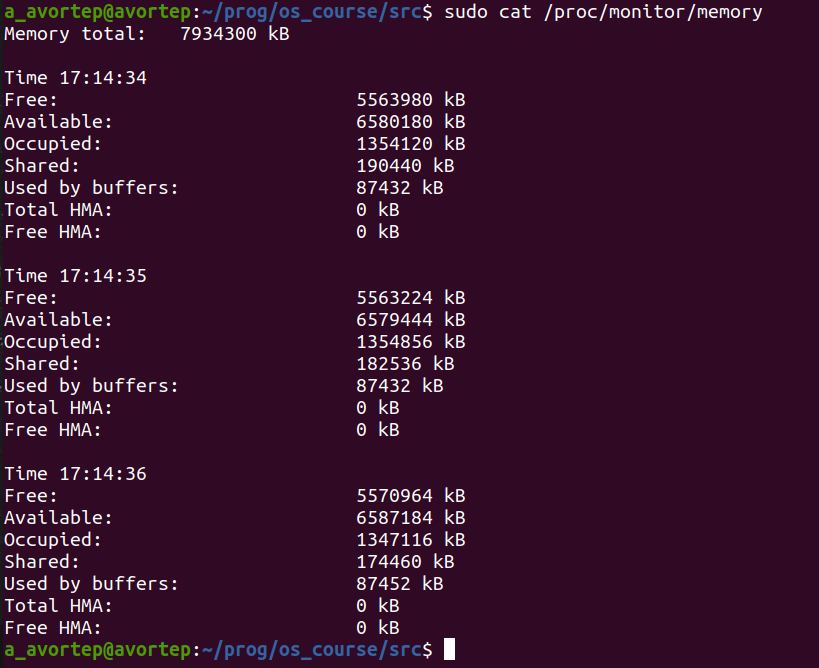
\includegraphics[scale=0.35]{jpg/mem_res.png}
	\end{center}
	\captionsetup{justification=centering}
	\caption{Информация об оперативной памяти в системе}
	\label{fig:example_mem}
\end{figure}

\begin{figure}[h!]
	\begin{center}
		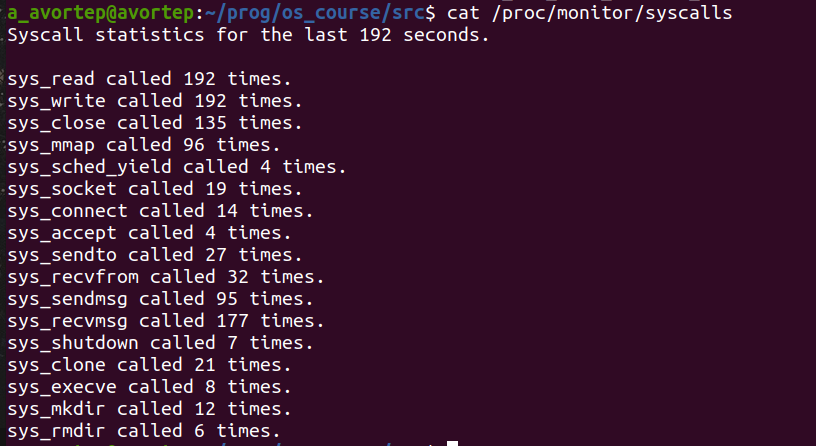
\includegraphics[scale=0.4]{jpg/cat_syscalls.png}
	\end{center}
	\captionsetup{justification=centering}
	\caption{Информация о количестве системных вызовов за последние 192 секунды}
	\label{fig:example_syscalls}
\end{figure}

На рисунке~\ref{fig:free-m} представлено сравнение результатов получения информации об объеме доступной и занятой оперативной памяти с результатами команды <<free -m>> (у последней все объемы указаны в Мб).

\begin{figure}[h!]
	\begin{center}
		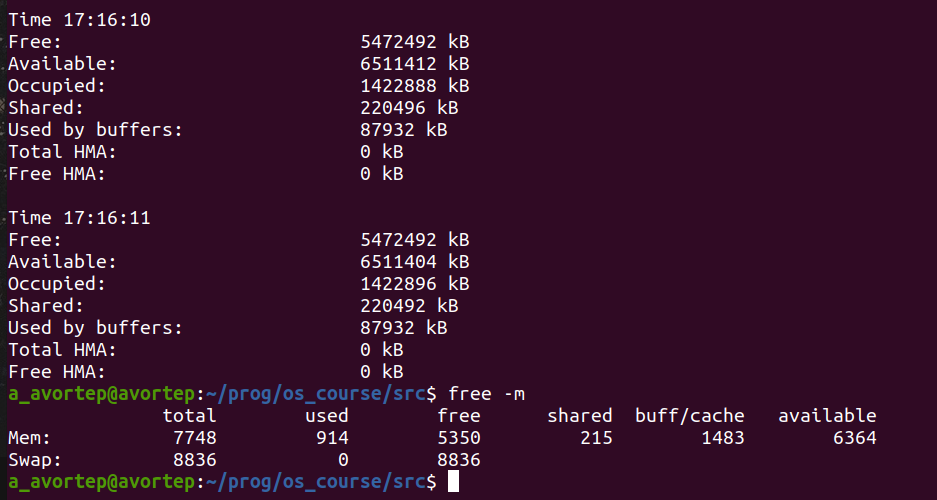
\includegraphics[scale=0.45]{jpg/free-m.png}
	\end{center}
	\captionsetup{justification=centering}
	\caption{Результаты работы команды <<free -m>>}
	\label{fig:free-m}
\end{figure}

Как видно из скриншота~\ref{fig:free-m}, результаты работы разработанного загружаемого модуля ядра близки к результатам работы команды <<free -m>>.

На рисунке \ref{fig:graphic} представлена визуализация данных о свободной, доступной и занятой памяти в системе, полученных из разработанного модуля ядра.

\begin{figure}[h!]
	\begin{center}
		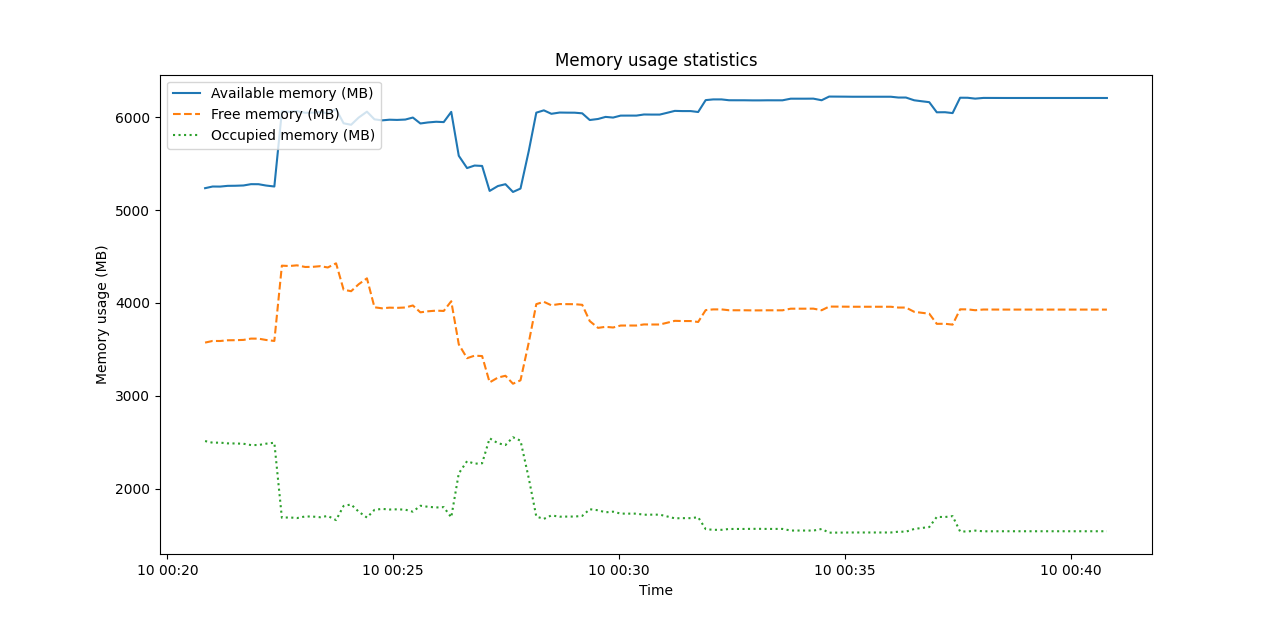
\includegraphics[scale=0.55]{jpg/memory_usage.png}
	\end{center}
	\captionsetup{justification=centering}
	\caption{Визуализация данных о памяти за 20 минут}
	\label{fig:graphic}
\end{figure}

\newpage

По графикам видно, как изменялась загруженность памяти в течение 20 минут. В моменты резкого спада количества занятой оперативной памяти было закрыто несколько приложений, а в моменты роста -- наоборот, открыто.

